% Template for Cogsci submission with R Markdown

% Stuff changed from original Markdown PLOS Template
\documentclass[10pt, letterpaper]{article}

\usepackage{cogsci}
\usepackage{pslatex}
\usepackage{float}
\usepackage{caption}

% amsmath package, useful for mathematical formulas
\usepackage{amsmath}

% amssymb package, useful for mathematical symbols
\usepackage{amssymb}

% hyperref package, useful for hyperlinks
\usepackage{hyperref}

% graphicx package, useful for including eps and pdf graphics
% include graphics with the command \includegraphics
\usepackage{graphicx}

% Sweave(-like)
\usepackage{fancyvrb}
\DefineVerbatimEnvironment{Sinput}{Verbatim}{fontshape=sl}
\DefineVerbatimEnvironment{Soutput}{Verbatim}{}
\DefineVerbatimEnvironment{Scode}{Verbatim}{fontshape=sl}
\newenvironment{Schunk}{}{}
\DefineVerbatimEnvironment{Code}{Verbatim}{}
\DefineVerbatimEnvironment{CodeInput}{Verbatim}{fontshape=sl}
\DefineVerbatimEnvironment{CodeOutput}{Verbatim}{}
\newenvironment{CodeChunk}{}{}

% cite package, to clean up citations in the main text. Do not remove.
\usepackage{apacite}

% KM added 1/4/18 to allow control of blind submission


\usepackage{color}

% Use doublespacing - comment out for single spacing
%\usepackage{setspace}
%\doublespacing


% % Text layout
% \topmargin 0.0cm
% \oddsidemargin 0.5cm
% \evensidemargin 0.5cm
% \textwidth 16cm
% \textheight 21cm

\title{Peekbank: Exploring child lexical processing through a large-scale
open-source database of developmental eyetracking datasets}


\author{{\large \bf Martin Zettersten (martincz@princeton.edu)} \\ Department of Psychology, South Dr \\ Princeton, NJ 08540 USA \AND {\large \bf CLinger Xu (txu@iu.edu)}  \AND {\large \bf Claire Bergey (cbergey@uchicago.edu)}  \AND {\large \bf Naiti S. Bhatt (nbhatt@hmc.edu)}  \AND {\large \bf Veronica Boyce (vboyce@stanford.edu)}  \AND {\large \bf Mika Braginsky (mikabr@mit.edu)}  \AND {\large \bf George Kachergis (kachergis@stanford.edu)}  \AND {\large \bf Molly Lewis (mollyllewis@gmail.com)}  \AND {\large \bf Jessica Mankewitz (jmankewitz@stanford.edu)} \AND {\large \bf Stephan Meylan (smeylan@mit.edu)}  \AND {\large \bf Annissa Saleh (ans638@nyu.edu)}  \AND {\large \bf Rose Schneider (roschnei@ucsd.edu)}   \AND {\large \bf Daniel Yurovsky (yurovsky@stanford.edu)}  \AND {\large \bf CMichael C. Frank (mcfrank@stanford.edu)}}


\begin{document}

\maketitle

\begin{abstract}
Developing lexical processing skills - the ability to rapidly process
words and link them to referents in context - is central to children's
early language development. Children's lexical processing is typically
studied in the looking-while-listening paradigm - also called the visual
world paradigm -, which measures infants' fixation of a target object
(as opposed to a distracter) after hearing a target label. In the
following paper, we present a large-scale open-source database of infant
and toddler looking-while-listening studies. The goal of this database
is to address theoretical and methodological challenges in measuring
infant vocabulary development that go beyond the scope of individual
studies. We present three preliminary analyses from the current
database: (1) models capturing item-level variability in infants'
lexical processing across age; (2) an analysis of how a central
methodological decision - selecting the time window of analysis -
impacts modeling results; (3) an analysis demonstrating the link between
the age of acquisition of specific words and children's ability to
rapidly and accurately link those words to their referents. Future
efforts will expand the scope of the current database to advance our
understanding of participant-level and item-level variation in
children's vocabulary development.

\textbf{Keywords:}
lexical processing; eyetracking; database; vocabulary development;
looking-while-listening; visual world paradigm
\end{abstract}

\hypertarget{introduction}{%
\section{Introduction}\label{introduction}}

Across their first years of life, children learn words in their native
tongues at a rapid pace. A key part of the word learning process is
children's ability to rapidly process words and link them to relevant
meanings in context - often referred to as lexical processing.
Developing lexical processing skills builds a foundation for children's
language development and is predictive of both linguistic and more
general cognitive outcomes later in life.

\hypertarget{the-success-of-the-looking-while-listening-paradigm}{%
\subsection{The success of the looking-while-listening
paradigm}\label{the-success-of-the-looking-while-listening-paradigm}}

Lexical processing is traditionally studied in
``looking-while-listening'' studies (sometimes called the intermodal
preference procedure). In such studies, infants listen to a sentence
prompting a specific referent (e.g., Look at the dog!) while viewing two
images on the screen (e.g., an image of a dog - the target image - and
an image of a duck - the distractor image). Infants' lexical processing
is measured in terms of how quickly and accurately infants subsequently
fixate the correct target image after hearing its label. Studies using
this basic design have contributed to our understanding of a wide range
of questions in language development, including infants' early noun
knowledge (Bergelson \& Swingley, 2012), phonological representations of
words (Swingley \& Aslin, 2000), prediction during language processing
(Lew-Williams \& Fernald, 2007), and individual differences in language
development (Marchman et al., 2018).

\hypertarget{outstanding-challenges}{%
\subsection{Outstanding challenges}\label{outstanding-challenges}}

While the looking-while-listening paradigm has been highly fruitful in
advancing understanding of early word knowledge, fundamental questions
remain both about the nature of children's early word knowledge and the
nature of the method itself. One central question relates to
understanding word-specific variability across development, and
generalizing lexical processing on the level of specific words. Most
studies of infant lexical processing focus on generalizing performance
across participants, and are constrained in their ability to provide
generalizations across the item level - the level of specific words.
Generalizing behavior on the level of both participants and items
simultaneously is often difficult in the context of a solitary study,
especially given practical constraints on the number of trials (and
consequently items) tested within a given infant. However, drawing
inferences about item-level variability is key to many questions in how
word learning unfolds, including how properties of the language input
influence lexical development (Item-based analytic approach - Goodman,
Dale, \& Li (2008), Roy et al.~(2015), Braginsky et al.~(2018) all look
at predicting items from input). One key to meeting this challenge is
having sufficiently large datasets to interrogate variability in lexical
processing on the item level.

A second question relates to evaluating methodological best-practices.
In particular, many fundamental analytic decisions vary substantially
across studies. For example, researchers vary in their decisions
regarding how to select time windows for analysis (XX), modeling how
lexical processing unfolds over time (XX), and the appropriate
transformations to perform on the dependent measure of target fixations.
Establishing best practices regarding analytic decisions of this kind
requires a large database of infant lexical processing studies, in order
to independently test the potential consequences of a variety of
methodological decisions on the interpretation of study results.

\hypertarget{peekbank-a-large-scale-database-of-looking-while-listening-studies}{%
\subsection{Peekbank: A large-scale database of
looking-while-listening-studies}\label{peekbank-a-large-scale-database-of-looking-while-listening-studies}}

What these questions and challenges share is that they are difficult to
answer at the scale of a single looking-while-listening study. In order
to address these questions, we introduce peekbank, a flexible and
reproducible interface to an open database of developmental eye-tracking
studies. Here, we give a brief overview over the key components of the
peekbank project and some initial demonstrations of its utility in
advancing theoretical and methodological questions in the study of
children's lexical processing. The peekbank project (a) collects a large
set of eye-tracking datasets on children's lexical processing, (b)
introduces a data format and processing tools for standardizing
eyetracking data across different data sources, and (c) provides an API
for quickly accessing and analyzing the database.

\hypertarget{methods}{%
\section{Methods}\label{methods}}

\hypertarget{database-framework}{%
\subsection{Database Framework}\label{database-framework}}

The Peekbank data framework consists of a relational database and two R
libraries: one to extract and rigorously validate data in preparation
for ingestion (peekds), and one that serves as an API that provides
high-level abstractions to run common analysis tasks on the database
(peekbankr).

The schema of the database (Fig. \#) is sufficiently general to handle
the dataset-specific parameters of datasets from many labs. Entities in
the schema include: subjects (an individual participant, who may
contribute to multiple datasets), administrations (a subject completing
a specific experiment), datasets (a data collection effort by a lab),
stimuli (a visual stimuli representing a common word, the label can be
in various languages), trials (a subject completing a specific trial),
trial\_types (metadata about a trial, which may be shared across
subjects), aoi\_region\_sets (areas of interest, linked to a specific
trial), aoi\_timepoints (coded looking behavior), xy\_timepoints (raw
looking behavior).

\hypertarget{current-data-sources}{%
\subsection{Current Data Sources}\label{current-data-sources}}

\begin{table}[H]
\centering
\begingroup\fontsize{9pt}{10pt}\selectfont
\begin{tabular}{lrrl}
  \hline
dataset\_name & num\_admin & avg\_age & method \\ 
  \hline
adams\_marchman\_2018 & 270 & 17.1 & manual coding \\ 
  casillas\_tseltal\_2015 & 23 & 31.3 & manual coding \\ 
  garrison\_bergelson\_2020 & 35 & 14.5 & eyetracking \\ 
  mahr\_coartic & 29 & 20.8 & eyetracking \\ 
  perry\_cowpig & 45 & 20.5 & manual coding \\ 
  pomper\_saffran\_2016 & 60 & 44.3 & manual coding \\ 
  pomper\_salientme & 44 & 40.1 & manual coding \\ 
  potter\_canine & 36 & 23.8 & manual coding \\ 
  reflook\_socword & 435 & 33.6 & eyetracking \\ 
  reflook\_v4 & 347 & 37.2 & eyetracking \\ 
   \hline
\end{tabular}
\endgroup
\caption{Overview over the datasets in the current database.} 
\end{table}

The database currently includes 10, ranging from 23 to 435 test sessions
per dataset. The vast majority of datasets consist of monolingual native
English speakers, with the exception of XX. The datasets span a wide age
range from X to Y and are balanced in terms of gender (m=XX\% female).
The studies in the current database vary across a number of dimensions
related to design and methodology. The database includes studies using
both manually coded video recordings or aumotated eyetracking methods to
measure children's gaze behavior. Most studies focused on testing
familiar items, but the database also includes studies in which both
familiar words and novel pseudowords were tested.

\hypertarget{data-processing}{%
\subsection{Data Processing}\label{data-processing}}

Resample to 40 ms

Process raw eyetracking datasets into unified ``AOA'' format focused on
looks at target or distracter (unified format for analysis across
manually coded and automated eyetracking data)

\hypertarget{results}{%
\section{Results}\label{results}}

\hypertarget{describing-variability-across-items}{%
\subsection{Describing Variability across
Items}\label{describing-variability-across-items}}

\begin{CodeChunk}
\begin{figure*}[h]

{\centering 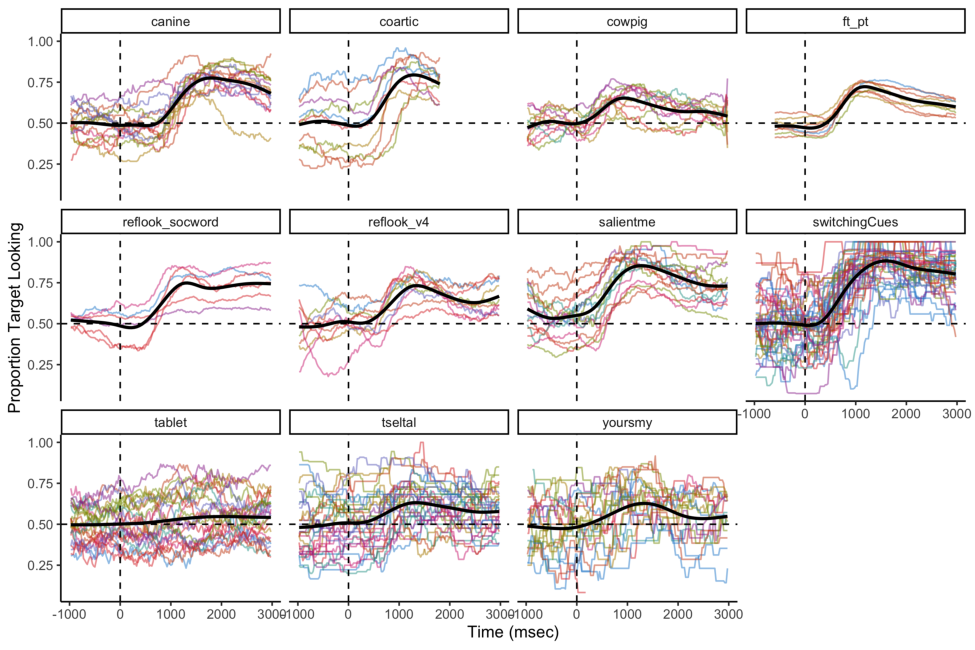
\includegraphics{figs/peekbank_item_vis-1} 

}

\caption[Item-level variability in proportion target looking within each dataset]{Item-level variability in proportion target looking within each dataset. Colored lines represent specific target labels.}\label{fig:peekbank_item_vis}
\end{figure*}
\end{CodeChunk}

\hypertarget{predicting-age-related-changes-while-generalizing-across-items}{%
\subsection{Predicting Age-Related Changes While Generalizing Across
Items}\label{predicting-age-related-changes-while-generalizing-across-items}}

Following the approach of Mirman (2014), we used growth curve modeling
to assess the timecourse of children's fixations to the target object at
different ages, generalizing across items. Specifically, we predicted
children's proportion of target looking during the critical window from
the interaction between age and four orthogonal polynomial time terms
(linear, quadratic, cubic, and quartic). We included by-item and
by-dataset random effects. Figure XX depicts the model fit at four
different age bins (though not that age was analyzed continuously in the
model).

We found that XXXXX.

\begin{CodeChunk}
\begin{figure}[H]

{\centering 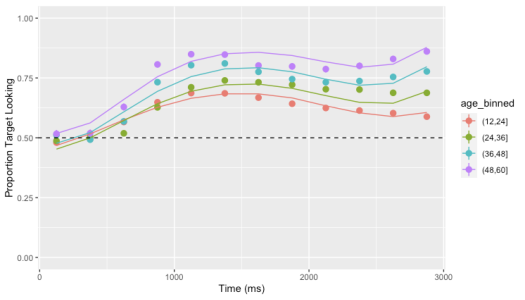
\includegraphics{figs/age_gca-1} 

}

\caption[Growth curve models of proportion target looking during the critical target window at each age range (in months)]{Growth curve models of proportion target looking during the critical target window at each age range (in months).}\label{fig:age_gca}
\end{figure}
\end{CodeChunk}

\hypertarget{predicting-target-fixation-from-word-aoa}{%
\subsection{Predicting Target Fixation from Word
AOA}\label{predicting-target-fixation-from-word-aoa}}

In the next analysis, we asked whether properties of a specific item -
in particular, the age of acquisition (AOA) for a particular item -
predict children's lexical processing. Using estimates of the age of
acquisition derived from Wordbank (Frank, Braginsky, Yurovsky, \&
Marchman, 2017) for the target and the distractor word, we modeled
whether earlier-acquired target words are more likely to be fixated
accurately. XX.

\hypertarget{time-window-selection}{%
\subsection{Time Window Selection}\label{time-window-selection}}

Following the approach of Peelle and Van Engen (2020), we conducted a
multiverse-style analysis considering possible time windows for
estimating the effect of age on proportion target looking in linear
mixed-effects models. In this analysis, we fit the same model across a
wide range of combinations of different start times for the critical
window (from XX ms pre target onset to XX ms post target word onset) and
window lengths (ranging from XX ms to XX ms). For each combination of
start time and window length, we fit a linear mixed-effects model
predicting proportion target looking from age, including random
intercepts for participants and words. Since observations were unevenly
distributed across the age range, we also split our data into three age
bins (12-24 months; 24-36 monts; 36-48 months).

Figure X visualizes the results of the mutliverse analysis, visualizing
the coefficient estimate and its associated p-value for each combination
of window start time and window length. As expected, proportion target
looking increases with age within each age time bin (as indicated by a
positive coefficient estimate). The analysis shows that the central
effect of age on proportion target looking is emerges under a wide range
of window choices. Intriguingly, each age range shows it's own ``hot
spot'' in terms of the largest effects: upper right for 12-24 mos,
bottom middle for 24-36 mos, and bottom right for 36-48 mos. This
suggests that researchers may be justified in using different start
times and window sizes for different age ranges, likely due to the
varying pull of familiarity and novelty as learners age.

\begin{CodeChunk}
\begin{figure*}[h]

{\centering 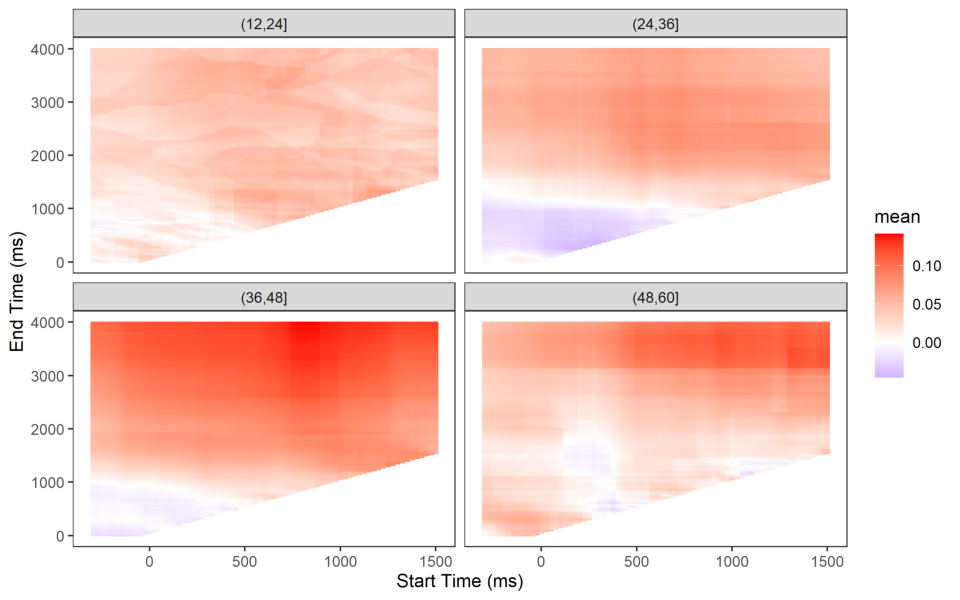
\includegraphics{figs/time_window-1} 

}

\caption[Time window analysis]{Time window analysis.}\label{fig:time_window}
\end{figure*}
\end{CodeChunk}

\hypertarget{discussion}{%
\section{Discussion}\label{discussion}}

Many central questions in developmental science face a fundamental data
collection challenge: Studying effects of interest requires a large
amount of observations, but collecting infant data is difficult,
time-intensive, and often limited to a small number of observations per
participant. Recent years have seen a growing effort to build open
source tools and pooling research efforts to meet the challenge of data
collection and aggregation in developmental science (Bergmann et al.,
2018; The ManyBabies Consortium, 2020). Peekbank expands on these
efforts by building an infrastructure for aggregating eyetracking data
across studies, with a particular focus on the looking-while-listening
paradigm. This paper presents a preliminary illustration of some of the
key theoretical and methodological questions the peekbank database aims
to address: understanding item-level variability in children's lexical
processing and providing data-driven guidance on methodological choices.

Diving into more specifics

Future directions and limitations

limitations in language background (almost entirely English,
monolingual)

limitations in participant background (almost entirely WEIRD
participants)

growing the database will address these questions while increasing our
power to answer the key generalization questions of interest

expanding beyond child lexical processing: tools and infrastructure can
in principle be expanded to accommodate any eyetracking paradigm used
with infants and toddlers

\hypertarget{acknowledgements}{%
\section{Acknowledgements}\label{acknowledgements}}

We would like to thank the labs and researchers that have made their
data publicly available in the database.

\hypertarget{references}{%
\section{References}\label{references}}

\setlength{\parindent}{-0.1in} 
\setlength{\leftskip}{0.125in}

\noindent

\hypertarget{refs}{}
\leavevmode\hypertarget{ref-Bergelson2012a}{}%
Bergelson, E., \& Swingley, D. (2012). At 6-9 months, human infants know
the meanings of many common nouns. \emph{Proceedings of the National
Academy of Sciences of the United States of America}, \emph{109}(9),
3253--8. \url{http://doi.org/10.1073/pnas.1113380109}

\leavevmode\hypertarget{ref-Bergmann2018}{}%
Bergmann, C., Tsuji, S., Piccinini, P. E., Lewis, M. L., Braginsky, M.,
Frank, M. C., \& Cristia, A. (2018). Promoting replicability in
developmental research through meta-analyses: Insights from language
acquisition research. \emph{Child Development}, \emph{89}(6),
1996--2009. \url{http://doi.org/10.1111/cdev.13079}

\leavevmode\hypertarget{ref-Frank2016}{}%
Frank, M. C., Braginsky, M., Yurovsky, D., \& Marchman, V. A. (2017).
Wordbank: An open repository for developmental vocabulary data.
\emph{Journal of Child Language}, \emph{44}(3), 677--694.
\url{http://doi.org/10.1017/S0305000916000209}

\leavevmode\hypertarget{ref-Lew-Williams2007}{}%
Lew-Williams, C., \& Fernald, A. (2007). Young children learning Spanish
make rapid use of grammatical gender in spoken word recognition.
\emph{Psychological Science}, \emph{18}(3), 193--198.
\url{http://doi.org/10.1111/j.1467-9280.2007.01871.x}

\leavevmode\hypertarget{ref-Marchman2018}{}%
Marchman, V. A., Loi, E. C., Adams, K. A., Ashland, M., Fernald, A., \&
Feldman, H. M. (2018). Speed of language comprehension at 18 months old
predicts school-relevant outcomes at 54 months old in children born
preterm. \emph{Journal of Developmental \& Behavioral Pediatrics}, 1.
\url{http://doi.org/10.1097/DBP.0000000000000541}

\leavevmode\hypertarget{ref-Mirman2014}{}%
Mirman, D. (2014). \emph{Growth curve analysis and visualization using
R}. CRC Press.

\leavevmode\hypertarget{ref-Peelle2020}{}%
Peelle, J. E., Engen, K. J. V., \& Sciences, B. (2020). Time stand
still: Effects of temporal window selection on eye tracking analysis.
\url{http://doi.org/https://doi.org/10.31234/osf.io/pc3da}

\leavevmode\hypertarget{ref-Swingley2000}{}%
Swingley, D., \& Aslin, R. N. (2000). Spoken word recognition and
lexical representation in very young children. \emph{Cognition},
\emph{76}(2), 147--66.

\leavevmode\hypertarget{ref-TheManyBabiesConsortium2020}{}%
The ManyBabies Consortium. (2020). Quantifying sources of variability in
infancy research using the infant-directed speech preference.
\emph{Advances in Methods and Practices in Psychological Science}.
\url{http://doi.org/10.1177/2515245919900809}

\bibliographystyle{apacite}


\end{document}
